\documentclass[12pt]{article}
\usepackage{graphicx}
\usepackage{listings}
\usepackage{algorithm,algpseudocode}
\usepackage{tikz}
\usepackage{amssymb}
\usepackage{lmodern}
\usepackage[colorlinks=false,plainpages=false,pdfborder={0 0 0},backref=false]{hyperref}


\lstset{frame=tb,
    aboveskip=3mm,
    belowskip=3mm,
    showstringspaces=false,
    columns=flexible,
    basicstyle={\small\ttfamily},
    numbers=none,
    numberstyle=\tiny\color{gray},
    keywordstyle=\color{blue},
    commentstyle=\color{dkgreen},
    stringstyle=\color{mauve},
    breaklines=true,
    breakatwhitespace=true,
    tabsize=3
}

\title{Evaluating Durability of Cloud Distributed Database: MongoDB Atlas}
\date{November 30th, 2020}
\author{Tiancheng(Zachary) Jin\\
SID:480187554\\
\\
Supervisor: Prof. Alan Fekete\\
Co-Supervisor: A/Prof. Uwe Roehm, Michael Cahill
}

\begin{document}
\newcommand{\algorithmautorefname}{Algorithm}
\maketitle
\newpage
\section{Introduction}
MongoDB, as one of the leading fault-tolerant NoSQL databases, has been widely used in recent years due to its high performance and scalability compared with the relational databases of the same scale, attracting many large enterprises and small start-up businesses who expect to access the data all around the world to purchase the databases as a service(DBaaS). MongoDB sought to fill this need by offering MongoDB Atlas, the cloud-based database service that let users access the database platform without setting up their own physical hardware and database software, along with managing the configuration of the databases \hyperref[sec:reference]{(IBM, 2019)}.\\
\\
As MongoDB Atlas is a fully managed distributed system using MongoDB, one of the properties it must guarantee to provide is durability. Durability is part of ACID properties for database transactions, ensuring the transaction remains committed in the database after it has been committed even if a server failure occurs \hyperref[sec:reference]{(Haerder \& Reuter, 1983)}. Without durability, data stored may be incorrect and lost when there is a failure.\\
\\
Our research is based on the previous research presented by \hyperref[sec:reference]{Konstatine Dunn(2018)}. In his research thesis, performance and durability properties were measured under different configuration choices, by deliberately causing failures of the servers. However, MongoDB servers were running on 3 virtual machines within one computer from his experiment, which is different from the real world settings that MongoDB servers are deployed into separate virtual machines using cloud services as what MongoDB Atlas does to provide the database services. To solve this limitation, experiments have been performed in this research to test whether MongoDB servers still maintain durability when they are deployed to the realistic cloud configurations.\\
\\
\section{Background}
\subsection{MongoDB \& MongoDB Atlas}
MongoDB is an open-source NoSQL database program initially released in 2009. Apart from relational databases that have fixed table structures and schemas, MongoDB holds collections of JSON-like documents with dynamic schemas, where collection is the equivalent of table and document is the equivalent of row in relational databases \hyperref[sec:reference]{(Singh, 2020)}. This feature makes MongoDB more flexible to access and store the data as the number of fields can be different between documents.\\
\\
WiredTiger is the default storage engine of MongoDB, providing snapshots of data to the operation for data consistency. WiredTiger also uses a write-ahead log (i.e. journal) to make data durable \hyperref[sec:reference]{(WiredTiger Storage Engine, 2020)}. If the journal option is enabled, modified data will be first recorded in journal, and then flush to the hard disk of database. \\
\\
Since MongoDB is only a database program, if the users want to use the database, they are required to configure and manage the MongoDB database. However, MongoDB Atlas, which is a fully managed database service using cloud services such as cloud computing and database storage, offers MongoDB as a service. People can spend more time building apps than managing databases\hyperref[sec:reference]{(Managed MongoDB Hosting, 2020)}. MongoDB Atlas deploys and manages MongoDB servers with different choices of cloud providers: AWS, Google Cloud, and Azure. \\
\subsection{AWS}
Amazon Web service(AWS) is a secure cloud services platform, offering cloud computing, database storage and other functionalities. Amazon Elastic Compute Cloud(EC2) is one of the web services in AWS that provides users with cloud virtual machines to perform secure cloud computing. MongoDB Atlas deploys and manages MongoDB servers on separate AWS EC2 machines.\\
\\
Among the AWS EC2 virtual machines, in order to let them communicate with each other under the secure environment, Amazon Virtual Private Cloud(Amazon VPC) provisions a isolated virtual network for the AWS launched resources\hyperref[sec:reference]{(VPC, 2020)}. MongoDB servers are allowed to be deployed at different Availability Zones that are isolated locations in the VPC, and each of the MongoDB servers can send messages to and receive messages from other servers by accessing the private IP addresses within the same VPC. The private IP addresses cannot be visited from the outside internet while we can connect to the EC2 virtual machines by using their public IP addresses.\\
\subsection{Replication}
MongoDB is able to provide high availability with replica sets to achieve fault-tolerance. A MongoDB replica set has at least 2 MongoDB instances and each has the same copy of the data. Each instance in the replica set has one of 2 different roles: either primary or secondary replica. By default, all writes and reads are handled by one single primary replica in a replica set. The remaining replicas are the secondary replicas that are responsible for read operation only.\\
\\
Once the primary replica receive write operations from clients, it will send those update information to secondary replicas to maintain identical data via Oplog. The Oplog contains a record of all the operations that modify the data and secondary replicas can continously apply the Oplog sent from primary replica to keep data updated and consistent.\\
\\
\begin{figure}
  \centering
  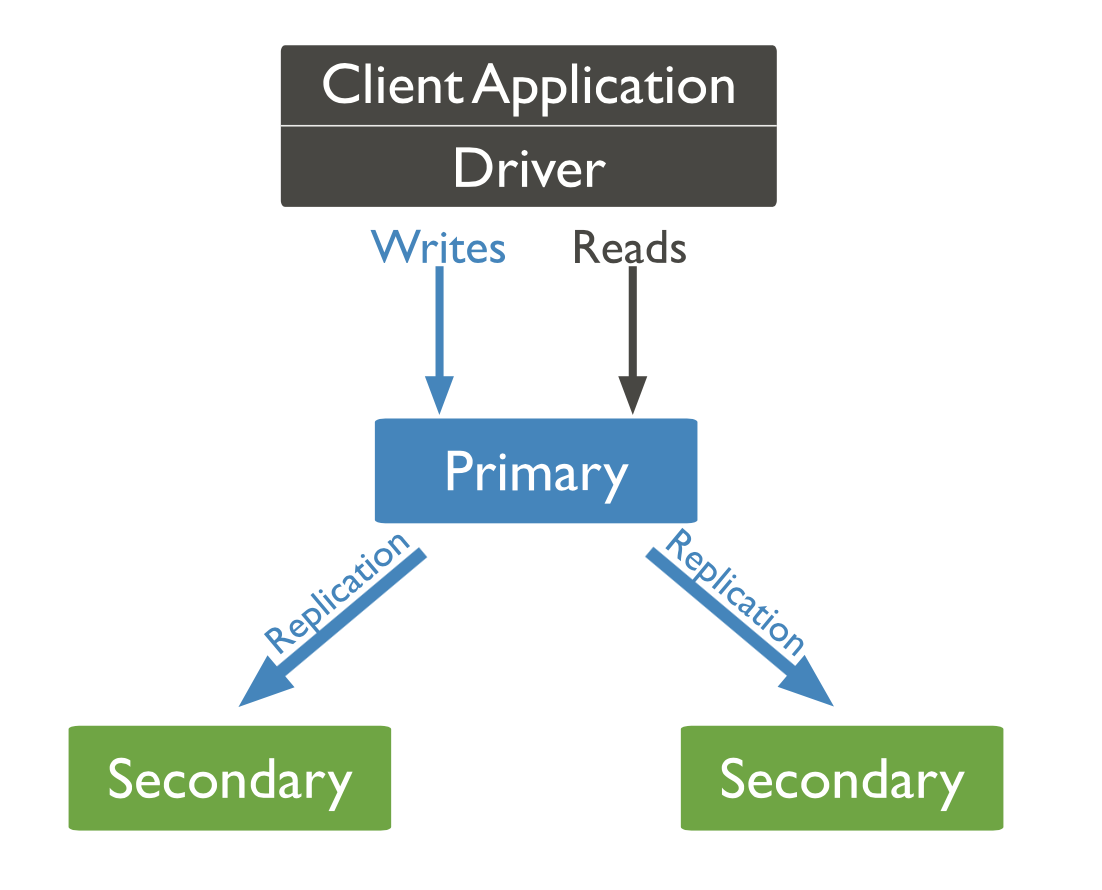
\includegraphics[width=0.5\textwidth, height=50mm]{img/replica.png}
  \caption{MongoDB replica set \hyperref[sec:reference]{(Replication for MongoDB, 2020)}}
  \label{fig:replica}
\end{figure}
\subsection{Election After Failure}
Among the members in the replica set, MongoDB servers use a simple heartbeat scheme to detect if their neighbours are still alive. The scheme can immediately find out the replica that is experiencing server failure and the replica set disconnects that failed replica temporarily.\\
\\
An election process will be conducted automatically to determine the primary replica in the replica set when the primary replica cannot be found by other replicas such as: the initial configuration stage or the moment when server failure affects the primary replica.\\
\\
We cannot guarantee that any server is always on and will not be down due to some failure. Failure is the inability of system to provide required functionality correctly \hyperref[sec:reference]{(Rashid, 2020)}. If the primary replica is down because of the failure, an election will be called soon to select a new primary since there is only one primary that can handle the write operations to the database system.\\
\\
\begin{figure}
  \centering
  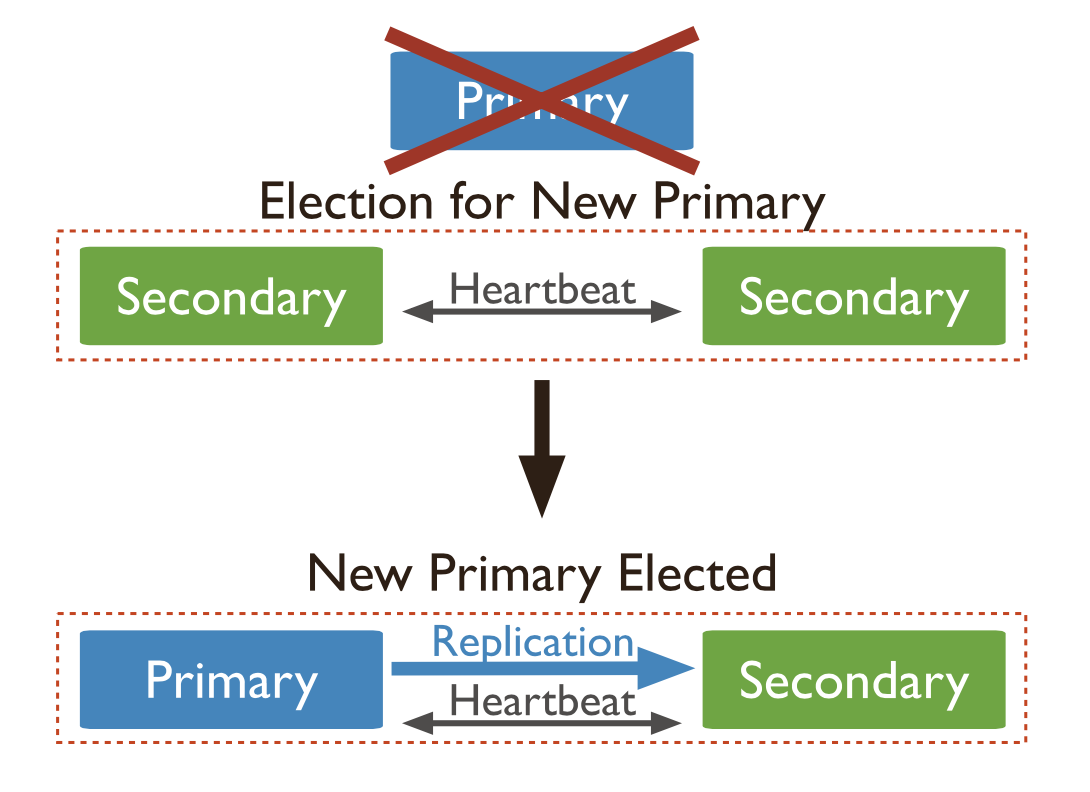
\includegraphics[width=0.5\textwidth, height=50mm]{img/fail.png}
  \caption{Automatic Failover \hyperref[sec:reference]{(Replication for MongoDB, 2020)}}
  \label{fig:fail}
\end{figure}
\subsection{Write Concern}
Write concern configured in MongoDB client defines the level of acknowledgement when the data is written to replica set, so that the client can know if the write operation is successful from the acknowledgement. In the experiment, we focus on 3 write concerns:\\
\begin{itemize}
  \item \textbf{Primary}: Acknowledge the writes right after the primary replica applies the operation
  \item \textbf{Journaled}: Acknowledge the writes after primary journal has obtained the operation
  \item \textbf{Majority}: Acknowledge the writes until more than half of the members in the replica set acknowledge
\end{itemize}
\subsection{Read Concern}
Read concern configured in MongoDB client defines how the data is read from servers for data consistency. In the experiment, we focus on 2 read concerns:\\
\begin{itemize}
  \item \textbf{Local}: Return the data from one of the members directly
  \item \textbf{Majority}: Return the data that has been acknowledged by more than half of the members in the replica set
\end{itemize}
\subsection{Read Preference}
Read preference configured in MongoDB client defines which replica we can send read operations to. In the experiment, we focus on 2 read preferences:\\
\begin{itemize}
  \item \textbf{Primary}: All the read operations are performed on primary replica
  \item \textbf{Primary Preferred}: Read operations are performed on primary replica, but if it is unavailable, read operations are performed on secondary replicas
\end{itemize}
\section{Aims}
The aim of our research is to perform an experiment to test and measure the durability of MongoDB Atlas, the cloud hosted system, with 2 different versions of MongoDB, allowing users and system developers to understand and increase the durability of MongoDB Atlas. Separate experiments need to be performed under various configurations and failures since the durability varies depending on those settings for write operations.\\
\\
The test harness for our experiment is based on the measurement method from the thesis written by \hyperref[sec:reference]{Dunn(2018)}, which uses only major operations that appears in all the NoSQL databases. We need to update the previous harness with Java programming language because we only find the Java API that can control the AWS machines.\\
\\
Besides, we also need to conduct an analysis of how certain configuration affects the writes durability within the replica set of MongoDB Atlas from the execution history, and determine whether the conclusion made in the previous Dunn's research also holds for this cloud-hosted system. \\
\\
There exist several challenges during the experiment. One challenge is that MongoDB Atlas cloud services cannot be shut down internally. Since MongoDB Atlas is fully managed by cloud provider, it is impossible for a normal user to control and induce the failures using framework from the user side. Therefore, we need to find a way to design a cloud-based system where we can cause server failures to MongoDB deployed on cloud, which becomes another challenge in the experiment since we are required to configure and manage the database server manually on cloud services to simulate the environment of MongoDB Atlas.\\
\\
\section{Methods}
At the initial stage of our research, several attempts have been made on finding a solution to send the failure signals to the MongoDB Atlas cluster from our test framework at the client side(our local computer). However, as the MongoDB Atlas cloud system is providing the database services to the users and users are not allowed to manage the internal MongoDB replica set by themselves, we failed to design the experiment by simply deploying the databases to MongoDB Atlas system. Due to this limitation of inducing failures to the MongoDB Atlas cloud system, we decided to directly deploy and manage the MongoDB servers on AWS virtual machines. This step is to simulate the environment of MongoDB Atlas using infrastructure as a service since AWS is one of the cloud providers for MongoDB Atlas.\\
\\
After the configuration of MongoDB servers on separate AWS virtual machines, MongoDB servers can automatically be turned on when we start the AWS virtual machines and similarly, they can stop working once the virtual machines are stopped. We also successfully found a method to send the shutdown and poweroff signals to the AWS virtual machines by using a Java API, which indicates that we can induce the server failures within our test framework during the experiment.\\
\\
We developed and updated the client application framework to send data requests automatically to the database in production during the experiment. Based on the execution history collected from the experiment, we can quantitatively evaluate the durability of MongoDB Atlas by measuring frequency of write losses under different configurations and failures.\\
\subsection{Server Setup in AWS}
To design a cloud-based system where we can cause server failures, MongoDB replica sets have been created and configured manually in AWS EC2 virtual machines. \\
\\
For each AWS EC2 virtual machine we launched, we selected \textit{Amazon Linux 2} AMI as the Amazon Machine Image containing the operating system. The instance type is \textit{m5.2xlarge} with 8 vCPUs and 32GB memory. We launched those virtual machine instances into the default Amazon Virtual Private Cloud(VPC) under different Availability Zone subnets.\\
\\
The MongoDB versions used in the experiment is 4.4, the current long-term support version as our control measurement and 3.6, the version with known durability problems. As shown below in the \hyperref[fig:instance]{\textit{figure 3}}, we set 3 EC2 machines for MongoDB 3.6 Community Edition and 3 EC2 machines for MongoDB 4.4 Community Edition so that we can perform experiments to see the durability improvement for MongoDB. There was also one EC2 machine, serving as the application that holds our test framework to stop and control the other machines inside the same VPC.\\
\\
Each machine contains a copy of data for MongoDB database. We connected to each of the mongo shell in each server and initiated the replica members. 3 MongoDB servers, together as one replica set, can communicate with each other within a private subnet by initiating their private IP addresses, which has the same \hyperref[fig:architecture]{\textit{architecture}} as the real world settings in MongoDB Atlas. \\
\begin{figure}
  \centering
  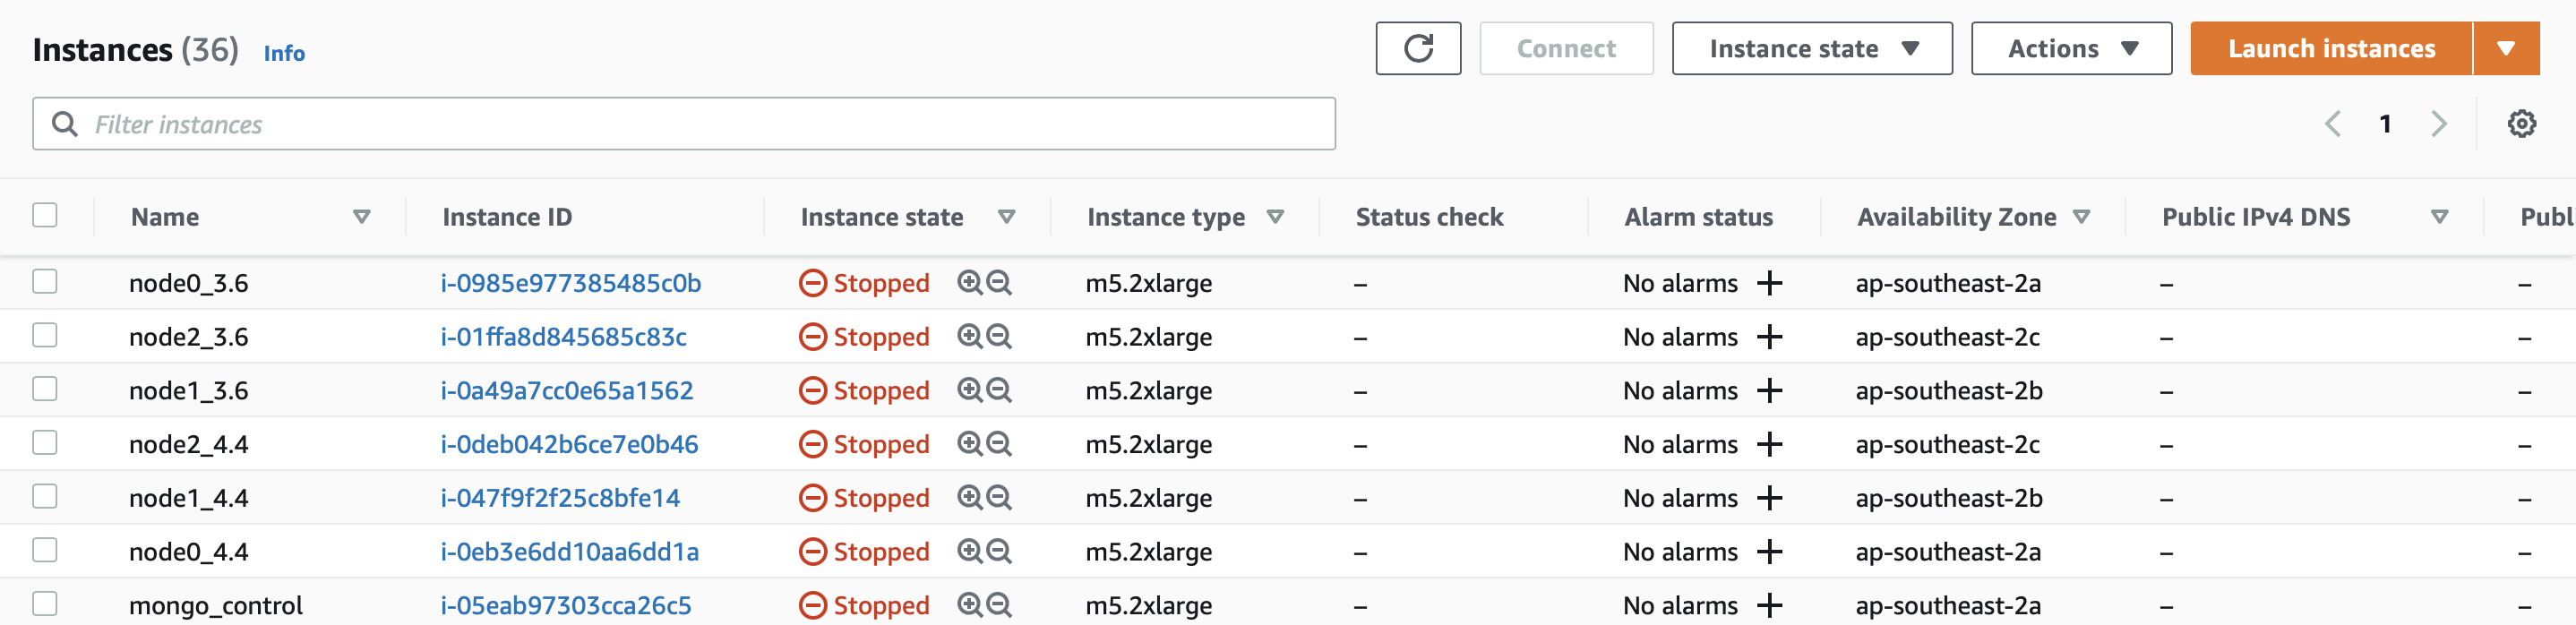
\includegraphics[width=\textwidth]{img/instance.png}
  \caption{7 launched VMs shown in AWS EC2 console}
  \label{fig:instance}
\end{figure}
\\
\begin{figure}
  \centering
  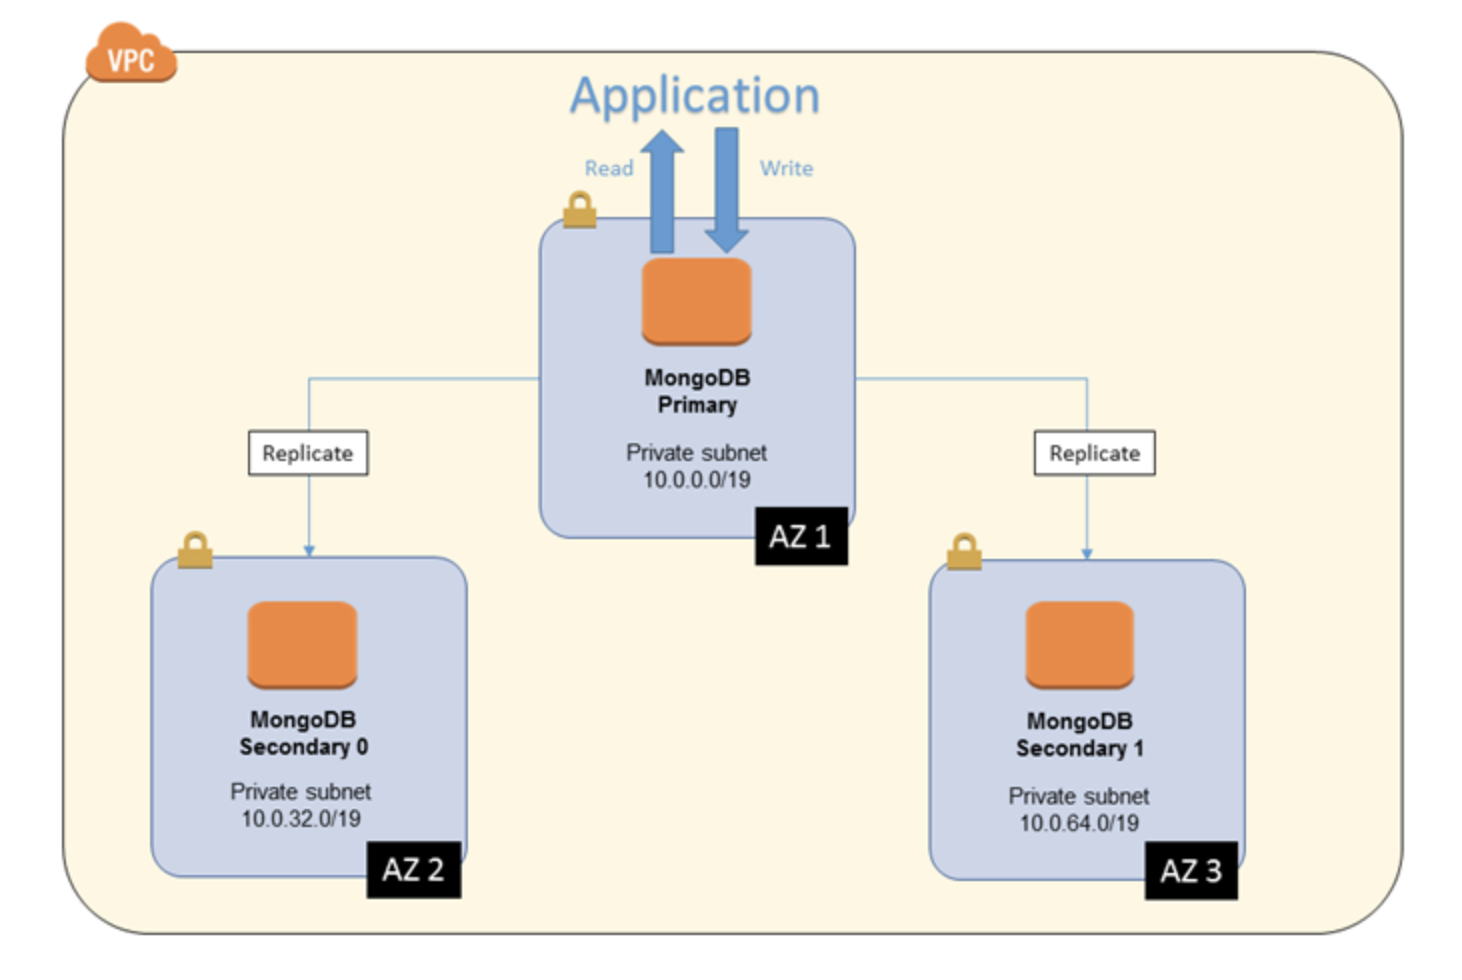
\includegraphics[width=0.8\textwidth, height=80mm]{img/architecture.png}
  \caption{Architecture - MongoDB on AWS\hyperref[sec:reference]{(Amazon Web Services Inc., 2020)}}
  \label{fig:architecture}
\end{figure}
\subsection{Inducing Failures}
The status of the MongoDB servers has been set to follow the status of AWS EC2 machines. Once the AWS machine is stopped, the MongoDB server will stop as well. When AWS machines restarts, the server will be turned on automatically. Therefore, in order to induce the failures to the MongoDB servers, we can make a call to control the AWS virtual machine. For the test framework, each failure was induced via a Java API call from AWS software development kit.\\
\\
In the experiment, we managed to induce the 2 server failures: Gracefully ACPI shutdown and Hard Poweroff to AWS EC2 machines.\\
\begin{itemize}
  \item \textbf{Gracefully ACPI shutdown}: Send ACPI shutdown signal, making the virtual machine shut down gracefully
  \item \textbf{Hard Poweroff}: Send Poweroff signal that turns off the virtual machine immediately
\end{itemize}
Since inducing failures to the secondary replica does not go through some recovery flow of the database system because secondary replica is only responsible for keeping copies of data and it is rare to raise durability issues here, the server failure was only induced to the primary replica as it is the only node who deals with the write operations from the client application. Before the previous primary replica has the chance to send the Oplog of some the data transactions to the secondary replicas, it is down due to some server failures, while the client has already received the acknowledgement messages from the previous primary replica. This may lead to the write losses related to the durability problems. \\
\\
Therefore, the steps to induce these 2 failures are as follows:
\begin{enumerate}
  \item Find the AWS instance with the current primary replica
  \item Create a java object for that AWS instance with class \textit{StopInstancesRequest} under package \textit{AmazonEC2Client}
  \item Invoke the \textit{setForce} method to set which failure will be induced. (Gracefully shutdown or poweroff)
  \item Call \textit{stopInstances} method to send the signal
  \item After the stage of operating under failure, restart the AWS instance by the java object with class \textit{StartInstancesRequest}
  \item Call \textit{startInstances} method to send the signal
\end{enumerate}
We can monitor the status of machines changing from running to stopped, and back to running on AWS EC2 console.\\
\subsection{Test Framework}
Each document stored in the database has the format of one simple id and an integer value as shown in \hyperref[alg:doc]{\textit{Algorithm 1}}.
\begin{algorithm}
\caption{Sample document stored in the database}
\begin{verbatim}
{
    id:  3,
    val: 9
}
\end{verbatim}
\label{alg:doc}
\end{algorithm}
\\
The measurement framework uses Java driver version 4.1 which is compatible with both MongoDB 4.4 and 3.6. We use this driver to make asynchronous interaction with MongoDB on AWS machines. A stress test is performed on 2 replica sets using this single client application with separate threads running concurrently. The harness can record all the operation commands sent to the database server and the error messages as an execution history.\\
\\
The duration of each experiment is 300 seconds. The experiment is divided into 3 stages:\\
\begin{itemize}
  \item \textbf{Standard stage}: At the start of the experiment, there are 100 seconds for the virtual machines to run in a normal manner.
  \item \textbf{Failure stage}: A failure is induced on the primary replica. The virtual machine holding this primary replica is shut down and it loses the connection with other members in the replica set.
  \item \textbf{Recovery stage}: The failed replica starts to run again and connect back to the replica set.
\end{itemize}
For each experiment, the workload of the test framework consists of 3 kinds of the NoSQL operations:\\
\begin{itemize}
  \item \textbf{Write operations(W)}: Append one document to the primary replica. The value in the document is assigned by a random integer generator.
  \item \textbf{Read operations(R)}: Randomly select an id from one existing document with acknowledged writes. Search for the document id and request its value. Any missing documents are considered as an error.
  \item \textbf{Update operations(U)}: Randomly select an id from one existing document with acknowledged writes. Search for the existing document id and write the new value to the document.
\end{itemize}
The harness can record all the operations and error messages with the timestamp of each event as one execution history file. The format of each record is shown in the \hyperref[fig:history]{\textit{figure 5}}. For each row, the record contains the operation type, document id, timestamp of this operation, the value inside the document, operation duration and the boolean value indicating whether there is an error.\\
\begin{figure}
  \centering
  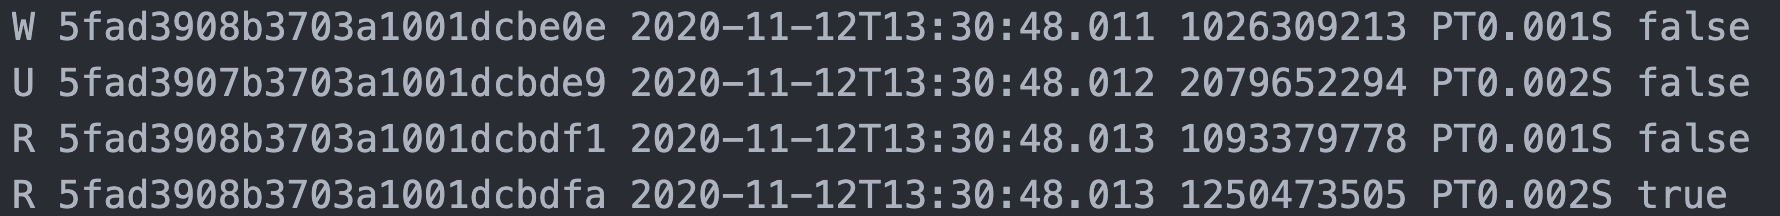
\includegraphics[width=\textwidth]{img/history.png}
  \caption{Sample records in execution history}
  \label{fig:history}
\end{figure}
\\
In the experiment, 10 threads are run as 10 actual users sent data records concurrently to the MongoDB servers through the Java driver program. Each of the thread performs individually with the replica set in parallel.\\
\\
There are 2 options: 0.7 and 0.3 for write probability that defines the percentage of write(including update) and read operations. For instance, 0.7 write probability means nearly 70 percent of the operations are writes and updates while only 30 percent are reads, testing the durability of a database that is more frequent to receive the queries for writing data.\\
\\
In addition, the configurations can also be set between various Read Concern, Write Concern and Read Preference. Those different options will largely affect the durability measurement result in the experiment. They can trade-off fault-tolerance for performance.\\
\subsection{Data Analysis}
Based on the execution history files generated from the experiments, data analysis produces the following attributes using \hyperref[alg:data]{\textit{Algorithm 2}}:\\
\begin{itemize}
  \item \textbf{Throughput}: The number of all successful operations
  \item \textbf{Errors}: The number of operations with negative acknowledgement
  \item \textbf{Lost Writes}: The number of write operations with positive acknowledgement but the data written are lost
\end{itemize}
\begin{algorithm}
\caption{Algorithm for data analysis}
\begin{verbatim}
op <- {}
success <- {}
errors <- {}
error_writes <- {}
lost_writes <- {}
unacknowledged_writes <- {}

for every record in execution history:
  if record.time <= failure.time:
    state <- normal
  else if failure.time <= record.time <= recovery.time:
    state <- failure
  else
    state <- recovery

  if record is error:
    add record to errors
    if record.operation == "W" or "U":
      add record to lost_writes
    end if
  else:
    add record to success
    if record.opration == "R":
      if record.value != op.expected:
        if record in errored_writes:
          add record to unacknowledged_writes
          delete record from errored_writes
        end if
      else:
        add record to lost_writes
      end if
    else:
      add (record.id, record.value) to op
    end if

  end if
end for
\end{verbatim}
\label{alg:data}
\end{algorithm}

\section{Results}
The measurement results are different between the previous research results with MongoDB deployed on local virtual machines, and our results with MongoDB deployed on 3 different virtual machines on cloud.\\
\\
Here are the experimental results under different configurations as mentioned in the Method section. \\
\\
\begin{table}
    \begin{tabular}{@{}lllccc@{}}
      \hline
        Read Preference  & Read Concern & Write Concern & Throughput & Errors & Lost Writes \\
        \hline
        Primary          & Local        & Primary       & 6911757     & 4  & 0        \\
        Primary          & Local        & Journaled     & 4256707     & 2  & 0        \\
        Primary          & Majority     & Majority      & 1746253     & 5  & 0           \\
        Primary Preferred & Local        & Primary       & 6802933     & 10   & 0        \\
        Primary Preferred & Local        & Journaled     & 2453044     & 2    & 0         \\
        Primary Preferred & Majority     & Majority      & 2169587     & 8   & 1           \\
        \hline
        \end{tabular}
    \caption{Experiment results MongoDB 4.4 with \textit{shutdown} failure on 0.3 write probability}
\end{table}

\begin{table}
    \begin{tabular}{@{}lllccc@{}}
      \hline
        Read Preference  & Read Concern & Write Concern & Throughput & Errors & Lost Writes \\
        \hline
        Primary          & Local        & Primary       & 6301731     & 8  & 0        \\
        Primary          & Local        & Journaled     & 1735878     & 5  & 0        \\
        Primary          & Majority     & Majority      & 1071242     & 7  & 2           \\
        Primary Preferred & Local        & Primary       & 6413355     & 9   & 0        \\
        Primary Preferred & Local        & Journaled     & 2347179     & 7    & 1         \\
        Primary Preferred & Majority     & Majority      & 952420     & 10   & 2           \\
        \hline
        \end{tabular}
    \caption{Experiment results MongoDB 4.4 with \textit{shutdown} failure on 0.7 write probability}
\end{table}

\begin{table}
    \begin{tabular}{@{}lllccc@{}}
      \hline
        Read Preference  & Read Concern & Write Concern & Throughput & Errors & Lost Writes \\
        \hline
        Primary          & Local        & Primary       & 6884372     & 4  & 0        \\
        Primary          & Local        & Journaled     & 2510398     & 4  & 0        \\
        Primary          & Majority     & Majority      & 1854392     & 6  & 4           \\
        Primary Preferred & Local        & Primary       & 9243531     & 3   & 0        \\
        Primary Preferred & Local        & Journaled     & 3203224     & 4    & 0         \\
        Primary Preferred & Majority     & Majority      & 2175725     & 5   & 1           \\
        \hline
        \end{tabular}
    \caption{Experiment results MongoDB 4.4 with \textit{poweroff} failure on 0.3 write probability}
\end{table}

\begin{table}
    \begin{tabular}{@{}lllccc@{}}
      \hline
        Read Preference  & Read Concern & Write Concern & Throughput & Errors & Lost Writes \\
        \hline
        Primary          & Local        & Primary       & 6388707     & 5  & 0        \\
        Primary          & Local        & Journaled     & 1717654     & 0  & 0        \\
        Primary          & Majority     & Majority      & 1124205     & 10  & 3           \\
        Primary Preferred & Local        & Primary       & 6292269     & 10   & 0        \\
        Primary Preferred & Local        & Journaled     & 1696288     & 2    & 0         \\
        Primary Preferred & Majority     & Majority      & 1118738     & 10   & 2           \\
        \hline
        \end{tabular}
    \caption{Experiment results MongoDB 4.4 with \textit{poweroff} failure on 0.7 write probability}
\end{table}

\begin{table}
    \begin{tabular}{@{}lllccc@{}}
      \hline
        Read Preference  & Read Concern & Write Concern & Throughput & Errors & Lost Writes \\
        \hline
        Primary          & Local        & Primary       & 9889812     & 1  & 0        \\
        Primary          & Local        & Journaled     & 3664291     & 6  & 0        \\
        Primary          & Majority     & Majority      & 1782030     & 10  & 0           \\
        Primary Preferred & Local        & Primary       & 7774638     & 10   & 0        \\
        Primary Preferred & Local        & Journaled     & 2728665     & 5    & 0         \\
        Primary Preferred & Majority     & Majority      & 1853176     & 10   & 3           \\
        \hline
        \end{tabular}
    \caption{Experiment results MongoDB 3.6 with \textit{shutdown} failure on 0.3 write probability}
\end{table}

\begin{table}
    \begin{tabular}{@{}lllccc@{}}
      \hline
        Read Preference  & Read Concern & Write Concern & Throughput & Errors & Lost Writes \\
        \hline
        Primary          & Local        & Primary       & 7255651     & 6  & 0        \\
        Primary          & Local        & Journaled     & 1854042     & 7  & 0        \\
        Primary          & Majority     & Majority      & 803808     & 9  & 1           \\
        Primary Preferred & Local        & Primary       & 7286117     & 10   & 0        \\
        Primary Preferred & Local        & Journaled     & 1691496     & 8    & 0         \\
        Primary Preferred & Majority     & Majority      & 909795     & 10   & 1           \\
        \hline
        \end{tabular}
    \caption{Experiment results MongoDB 3.6 with \textit{shutdown} failure on 0.7 write probability}
\end{table}

\begin{table}
    \begin{tabular}{@{}lllccc@{}}
      \hline
        Read Preference  & Read Concern & Write Concern & Throughput & Errors & Lost Writes \\
        \hline
        Primary          & Local        & Primary       & 7979853     & 5  & 0        \\
        Primary          & Local        & Journaled     & 2677525     & 2  & 0        \\
        Primary          & Majority     & Majority      & 1388192     & 10  & 7           \\
        Primary Preferred & Local        & Primary       & 7778215     & 10   & 0        \\
        Primary Preferred & Local        & Journaled     & 5121457     & 9    & 0         \\
        Primary Preferred & Majority     & Majority      & 1605661     & 10   & 2           \\
        \hline
        \end{tabular}
    \caption{Experiment results MongoDB 3.6 with \textit{poweroff} failure on 0.3 write probability}
\end{table}

\begin{table}
    \begin{tabular}{@{}lllccc@{}}
      \hline
        Read Preference  & Read Concern & Write Concern & Throughput & Errors & Lost Writes \\
        \hline
        Primary          & Local        & Primary       & 3450651     & 6  & 0        \\
        Primary          & Local        & Journaled     & 2652727     & 9  & 0        \\
        Primary          & Majority     & Majority      & 848675     & 10  & 2           \\
        Primary Preferred & Local        & Primary       & 3220748     & 9   & 0        \\
        Primary Preferred & Local        & Journaled     & 2672956     & 10    & 0         \\
        Primary Preferred & Majority     & Majority      & 866893     & 10   & 1           \\
        \hline
        \end{tabular}
    \caption{Experiment results MongoDB 3.6 with \textit{poweroff} failure on 0.7 write probability}
\end{table}
\section{Discussion}
What we have contributed in this research is that we successfully set up MongoDB servers on different machines on cloud services, allowing us to know how the MongoDB Atlas deploys and manages the database. We also learnt how to send shutdown signals to MongoDB remote servers from user sides by Java API. \\
\\
From the results shown above, the number of throughputs is nearly 10 times as the previous one for each of the experiment. Compared to the \hyperref[sec:reference]{Dunn's (2018)} results in his thesis, our experiments are closer to the real production using cloud services since the cloud services have more computing power that can handle more data requests at the same time than using a single laptop. Besides, as the throughputs increase, it is more possible to find out the potential durability issues in real life. \\
\\
However, lost writes in majority read and write concerns are not expected. As read and write concerns are both majority, indicating that for a data record in the database, a majority of the server must obtain its value if the write operation is successful, therefore lost writes are expected to be 0. However, non-zero values exist for lost writes from the 3th and 6th rows in each result table where the read and write concerns are both \textit{Majority}. For other configurations, we also found 0 lost writes in our results but those are possible based on the system structure.\\
\\
We will pay more efforts on researching internal Java driver program for MongoDB, which is the possible issue when connecting to the cloud virtual machine. We will continue our research to check if there exists a process for Java driver that if the acknowledgement message cannot be sent, the data record will not be stored.\\
\section{Conclusion}
The durability property of MongoDB servers can be measured in cloud settings, by self-managed servers to which faults are injected through API. For execution history analysis, the measurement results are obtained but they are different from the case of setting MongoDB servers on local virtual machines. The measured loss writes of durability are not aligned with expectations from the previous works on local machines, which requires us to perform more researches on this.\\
\section{Future Work}
There are several future works based on our research. We only used 2 versions of MongoDB replica set: version 4.4 and version 3.6. Different versions of MongoDB can be tested on durability to observe the performance and improvement as well. We only induce 2 types of server failures for crash-tolerant systems in the experiment. Other failures can also happen in real life and they can also be induced for testing.\\
\section{References}
\label{sec:reference}

[1] Amazon Web Services Inc. (2020). Architecture - MongoDB on AWS. (2020). Retrieved 25 November 2020, from https://docs.aws.amazon.com/quickstart
/latest/mongodb/architecture.html\\\relax
[2] Amazon Virtual Private Cloud (VPC). (2020). Retrieved 26 November 2020, from https://aws.amazon.com/vpc/ \\\relax
[3] Dunn, K. (2018). Evaluating Durability of Distributed
Databases: Theory and Empirical Studies of MongoDB, (Unpublished honour thesis), University of Sydney, Australia.\\\relax
[4] Haerder, T. \& Reuter, A. (1983). Principles of transaction-oriented database recovery. ACM Computing Surveys, 15(4):287–317. doi: 10.1145/289.291 \\\relax
[5] IBM Cloud Education. (2019). DBaaS(Database-as-a-Service). Retrieved 11 November 2020, from https://www.ibm.com/cloud/learn/dbaas \\\relax
[6] Managed MongoDB Hosting | Database-as-a-Service. (2020). Retrieved 26 November 2020, from https://www.mongodb.com/cloud/atlas \\\relax
[7] Rashid, H. (2020). Database Failure | Causes of Database Failure. Retrieved 26 November 2020, from https://limbd.org/database-failure-causes-of-database-failure/ \\\relax
[8] Replication — MongoDB Manual. (2020). Retrieved 26 November 2020, from https://docs.mongodb.com/manual/replication/ \\\relax
[9] Singh, C. (2020). Mapping Relational Databases to MongoDB. Retrieved 25 November 2020, from https://beginnersbook.com/2017/09/mapping-relational-databases-to-mongodb/ \\\relax
[10] WiredTiger Storage Engine — MongoDB Manual. (2020). Retrieved 26 November 2020, from https://docs.mongodb.com/manual/core/wiredtiger/ \\\relax

\section{Appendices}
All the source code for the experiment can be found in Github:\\
\href{https://github.com/zacharyjin8948/mongodbatlas\_durability.git}{https://github.com/zacharyjin8948/mongodbatlas\_durability.git}
\end{document}
